\documentclass{article}
\usepackage{graphicx}
\usepackage[margin=1.5cm]{geometry}
\usepackage{amsmath}
\usepackage{hyperref}
\hypersetup{
    colorlinks=true,
    linkcolor=blue,
    filecolor=magenta,      
    urlcolor=cyan,
    pdftitle={Overleaf Example},
    pdfpagemode=FullScreen,
}

\begin{document}
\twocolumn

\title{Thursday Warm Up, Unit 2: Applications}
\author{Prof. Jordan C. Hanson}
\maketitle

\section{Memory Bank}

\begin{enumerate}
\item \textbf{Point spread function (PSF)}. A two-dimensional filter kernel for image analysis.  Used with two-dimensional convolution to filter image data.
\end{enumerate}

\section{Linear Image Processing}

\begin{enumerate}
\item Download \textbf{\href{https://cms.whittier.edu/mod/resource/view.php?id=682787}{Image 1}} from our course Moodle page, dated April 17th. (b) Use the following code to load the image file in \verb+octave+:
\begin{verbatim}
data = imread('airport.png');
\end{verbatim}
\item (a) Print the size of the image data: \verb+size(data)+. (b) The pixels are labeled by row and column.  The RGB data stored at each pixel is redundant for this black and white image.  Check that the 3 values are equal for a variety of pixel values.  Equal RGB values indicate the color is on the grey scale.  (c) Discard all but one of the values, and make the image 450 by 450 pixels:
\begin{verbatim}
data = data(:,:,1);
data = data(1:450,1:450);
\end{verbatim}
\item Display the image with the \verb+imshow+ function.  Do you see anything interesting?  This image has low exposure; the pixel values are too dark.
\item Define a PSF (\verb+kernel+) that is a $3\times 3$ matrix, with the pattern in Fig. \ref{fig:1} (bottom).  That is, the central sample should be 1.0, while the others should be $-1/8$.
\item \textbf{Filter the image} using \verb+filter2+:
\begin{verbatim}
proc = filter2(kernel,data)
\end{verbatim}
Display the image with \verb+imshow+. Do you see the dangerous object?
\item Download the \textbf{\href{https://cms.whittier.edu/mod/resource/view.php?id=682804}{Image 2}} from our course Moodle page, dated April 17th. (b) Use the following code to load the image file in \verb+octave+:
\begin{verbatim}
data = imread('truck_license_plate_noise.png');
\end{verbatim}
\item (a) View the image using \verb+imshow+.  The driver of this truck is a \#@!7* and needs to go to jail.  Our task is to obtain the license plate number. (b) Define a $3\times 3$ filter kernel with ones in all samples, then divide it by the total number of samples. (c) Filter the image with the kernel, and isolate the pixels with the license plate. (d) Use \verb+flipud+ and \verb+fliplr+ to orient the plate so the markings are upright. (d) Write down the plate number:\underline{$~~~~~~~~~~~~~~~~~~~~~~~~~~~~~~$}.
\end{enumerate}

\begin{figure}
\centering
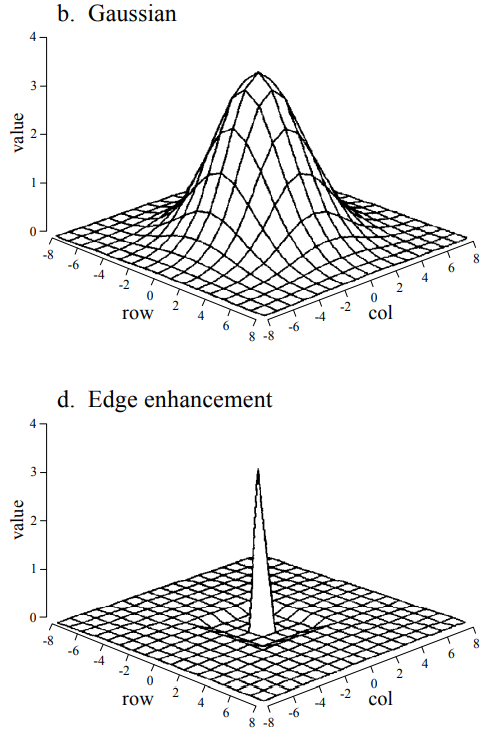
\includegraphics[width=0.45\textwidth]{image_PSF.png}
\caption{\label{fig:1} PSFs used in image smoothing.}
\end{figure}

\end{document}
